\documentclass[12pt]{article}
\usepackage[svgnames,x11names,table]{xcolor}
\usepackage{hyperref}
\usepackage{graphicx}
\usepackage{parskip}
\usepackage{float}
\usepackage{amsmath}
\usepackage{amssymb}
\usepackage{enumitem}
\usepackage[thicklines]{cancel}

\hypersetup{
    colorlinks,
    citecolor=black,
    filecolor=black,
    linkcolor=RoyalBlue4,
    urlcolor=RoyalBlue4,
}

\title{PEU 356 Assignment 1}
\author{Mohamed Hussien El-Deeb (201900052)}
\date{\today}

\begin{document}

\maketitle
\tableofcontents

\section{3.10.1}

\subsection{Problem}

The \(u-, v-, z-\)coordinate system frequently used in electrostatics and in hydrodynamics
is defined by

\[
    xy = u, x^2 - y^2 = v, z = z
\]

This \(u-, v-, z-\)system is orthogonal.
\bigskip

\begin{enumerate}[label= \textbf{(\alph*)}]
    \item In words, describe briefly the nature of each of the three families of coordinate
          surfaces.
    \item Sketch the system in the \(x y-\)plane showing the intersections of surfaces of constant
          u and surfaces of constant v with the \(x y-\)plane.
    \item Indicate the directions of the unit vectors \(\hat{\mathbf{e}}_u\) and \(\hat{\mathbf{e}}_v\)
          in all four quadrants.
    \item Finally, is this \(u-, v-, z-\)system right-handed \((\hat{\mathbf{e}}_u \times \hat{\mathbf{e}}_v
          = +\hat{\mathbf{e}}_z )\) or left-handed \((\hat{\mathbf{e}}_u \times
          \hat{\mathbf{e}}_v = -\hat{\mathbf{e}}_z )\)?
\end{enumerate}

\subsection{Solution}

\subsubsection{a}

\(u\) curves are \(\frac{n}{x}\) asymptotes, \(u=0\) is xz-plane, repeated for all values of \(z\).

\[
    (x, \frac{u_i}{x}, z)
\]

\(v\) curves are x shaped for \(v=0\), horizontal hyperbola for \(v>0\), vertical hyperbola for
\(v<0\), repeated for all values of \(z\).

\[
    (x, \pm\sqrt{x^2 - v_i}, z)
\]

\(z\) curves are planes parallel to xy-plane.


\[
    (x, y, z_i)
\]

\subsubsection{b}

\begin{figure}[H]
    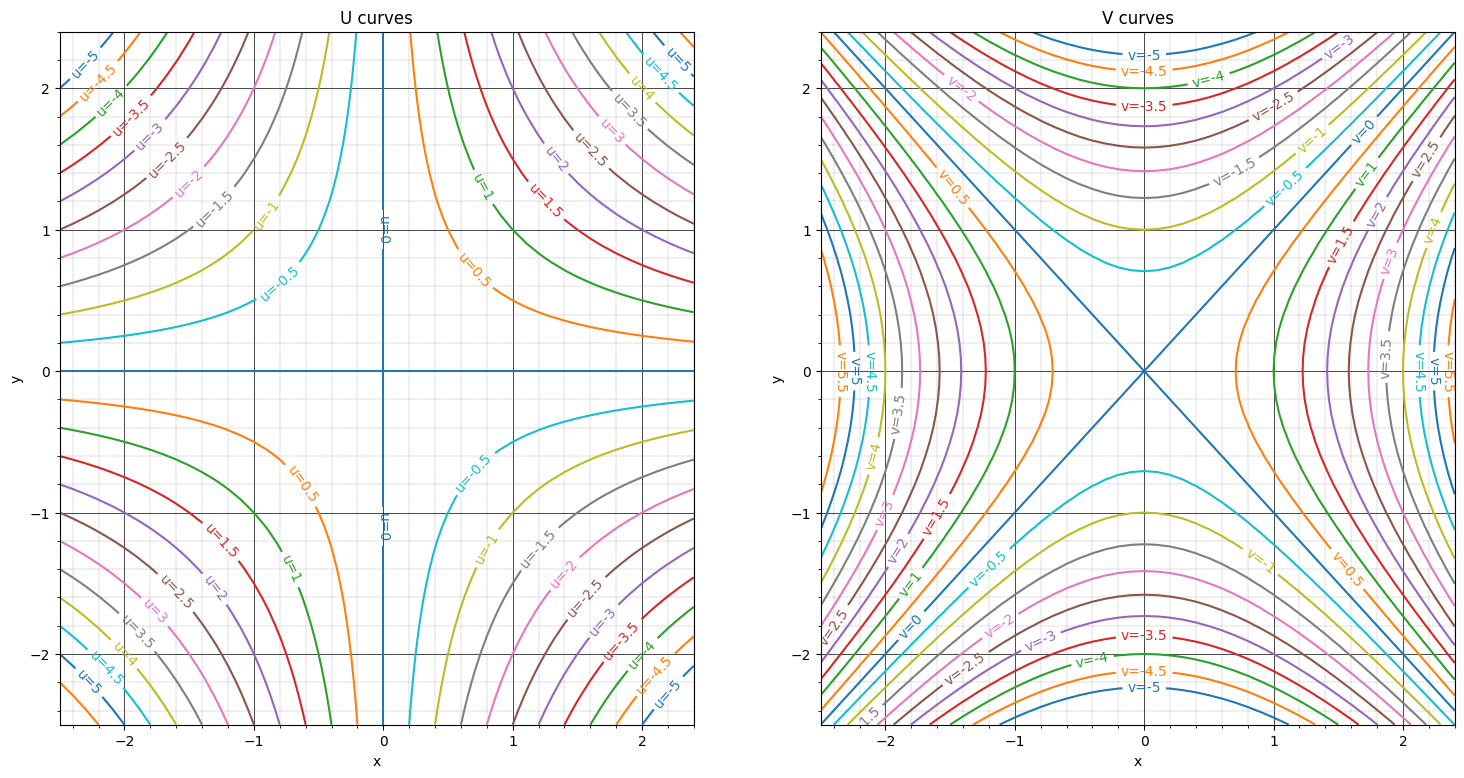
\includegraphics[width=\linewidth]{Q1B.png}
    \caption{U and V curves.}\label{fig:Q1B}
\end{figure}

\begin{figure}[H]
    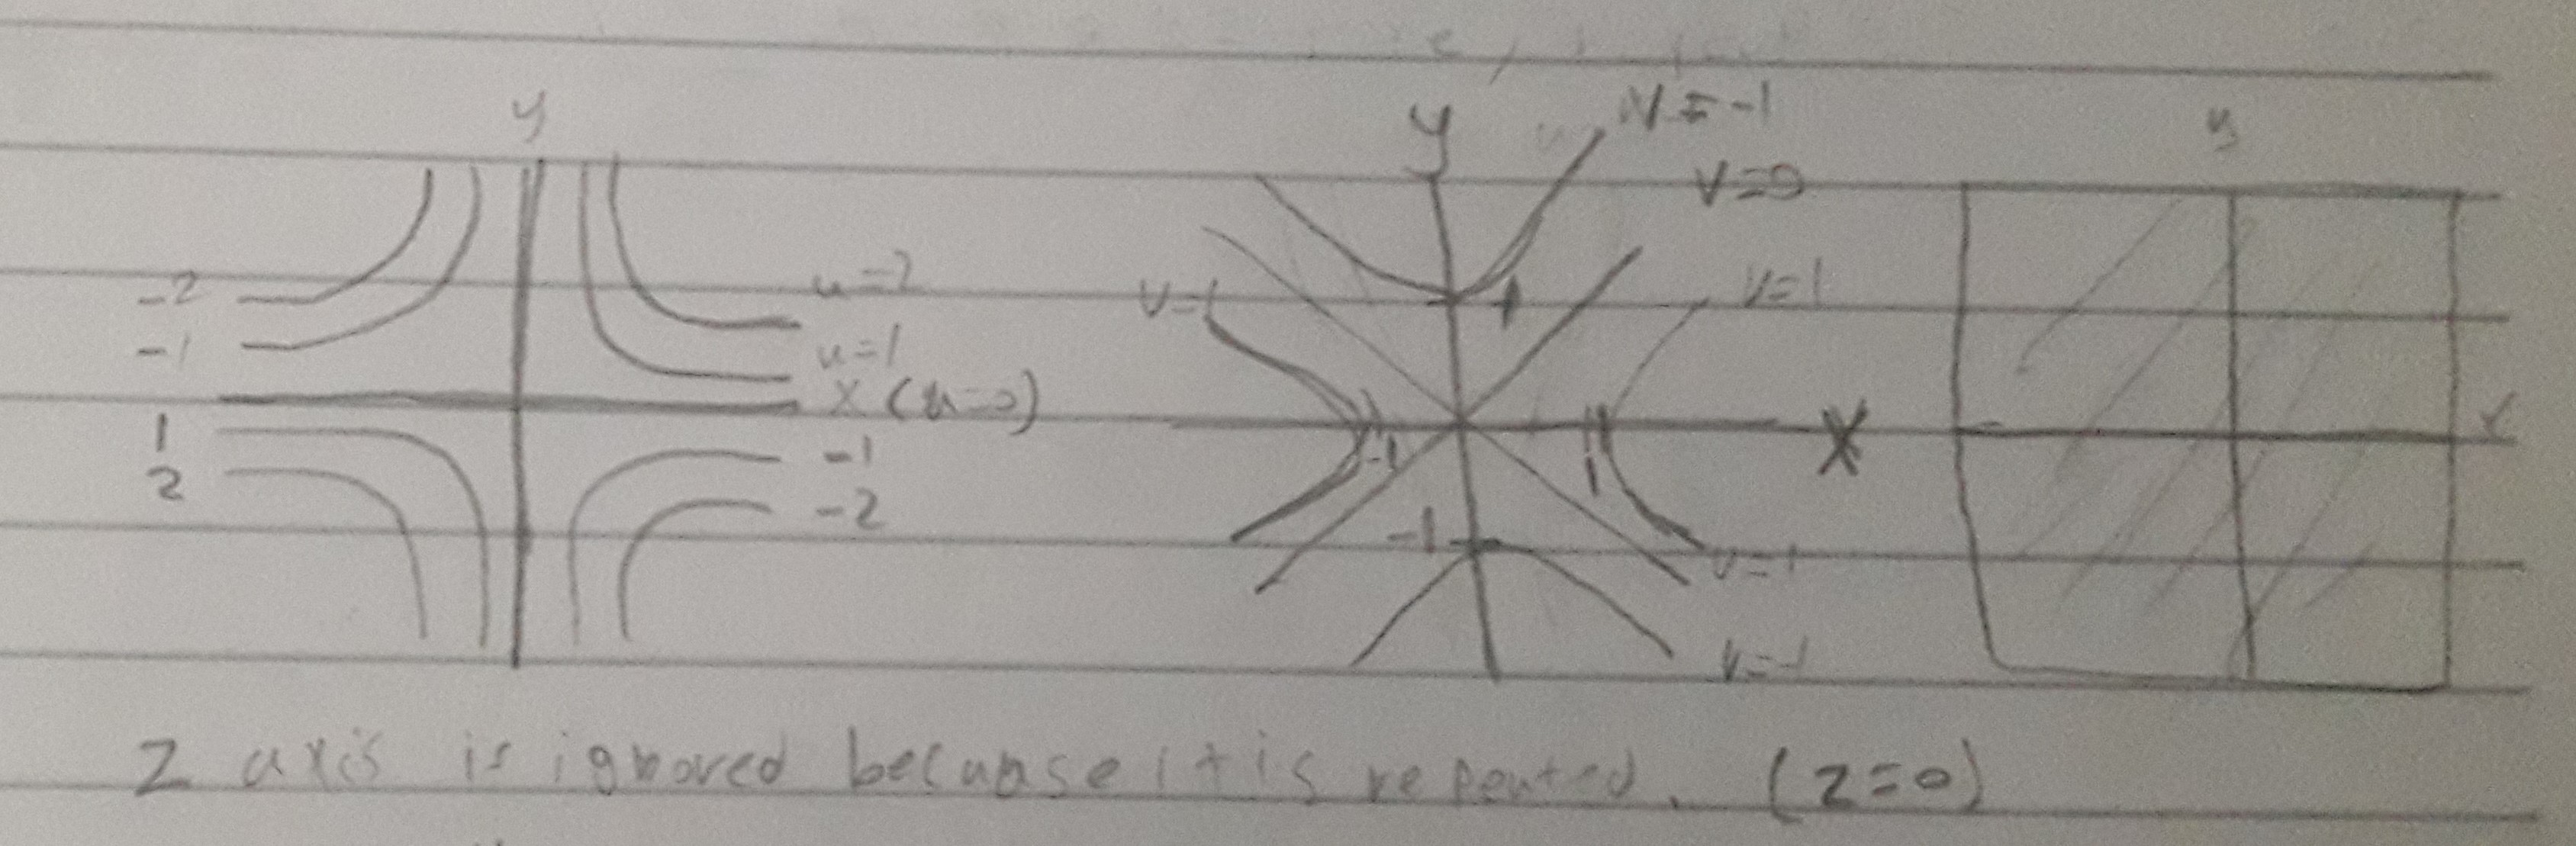
\includegraphics[width=\linewidth]{Q1B.jpg}
    \caption{U and V curves sketch.}\label{fig:Q1B2}
\end{figure}

\subsubsection{c}

\[
    \nabla u = \frac{ \partial u}{\partial x} \hat{\dot{\imath}}
    + \frac{ \partial u}{\partial y}  \hat{\dot{\jmath}} = \frac{ \partial (xy)}{\partial x}  \hat{\dot{\imath}}
    + \frac{ \partial (xy)}{\partial y}  \hat{\dot{\jmath}} = y  \hat{\dot{\imath}}
    + x  \hat{\dot{\jmath}}
\]

\[
    \nabla v = \frac{ \partial v}{\partial x} \hat{\dot{\imath}}
    + \frac{ \partial v}{\partial y}  \hat{\dot{\jmath}}
    = \frac{ \partial (x^2 - y^2)}{\partial x}  \hat{\dot{\imath}}
    + \frac{ \partial (x^2 - y^2)}{\partial y}  \hat{\dot{\jmath}}
    = 2x  \hat{\dot{\imath}} - 2y  \hat{\dot{\jmath}}
\]

\[
    \hat{\mathbf{e}}_u = \frac{\nabla u}{|\nabla u|} = \frac{y  \hat{\dot{\imath}}
        + x  \hat{\dot{\jmath}}}{\sqrt{x^2 + y^2}}
\]

\[
    \hat{\mathbf{e}}_v = \frac{\nabla v}{|\nabla v|} = \frac{2x  \hat{\dot{\imath}}
        - 2y  \hat{\dot{\jmath}}}{\sqrt{4x^2 + 4y^2}}
\]

\begin{figure}[H]
    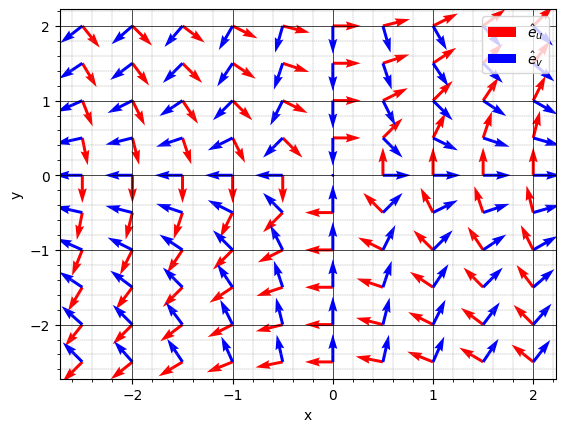
\includegraphics[width=\linewidth]{Q1C.png}
    \caption{Basis Vectors Field Plot}\label{fig:Q1C}
\end{figure}

\begin{figure}[H]
    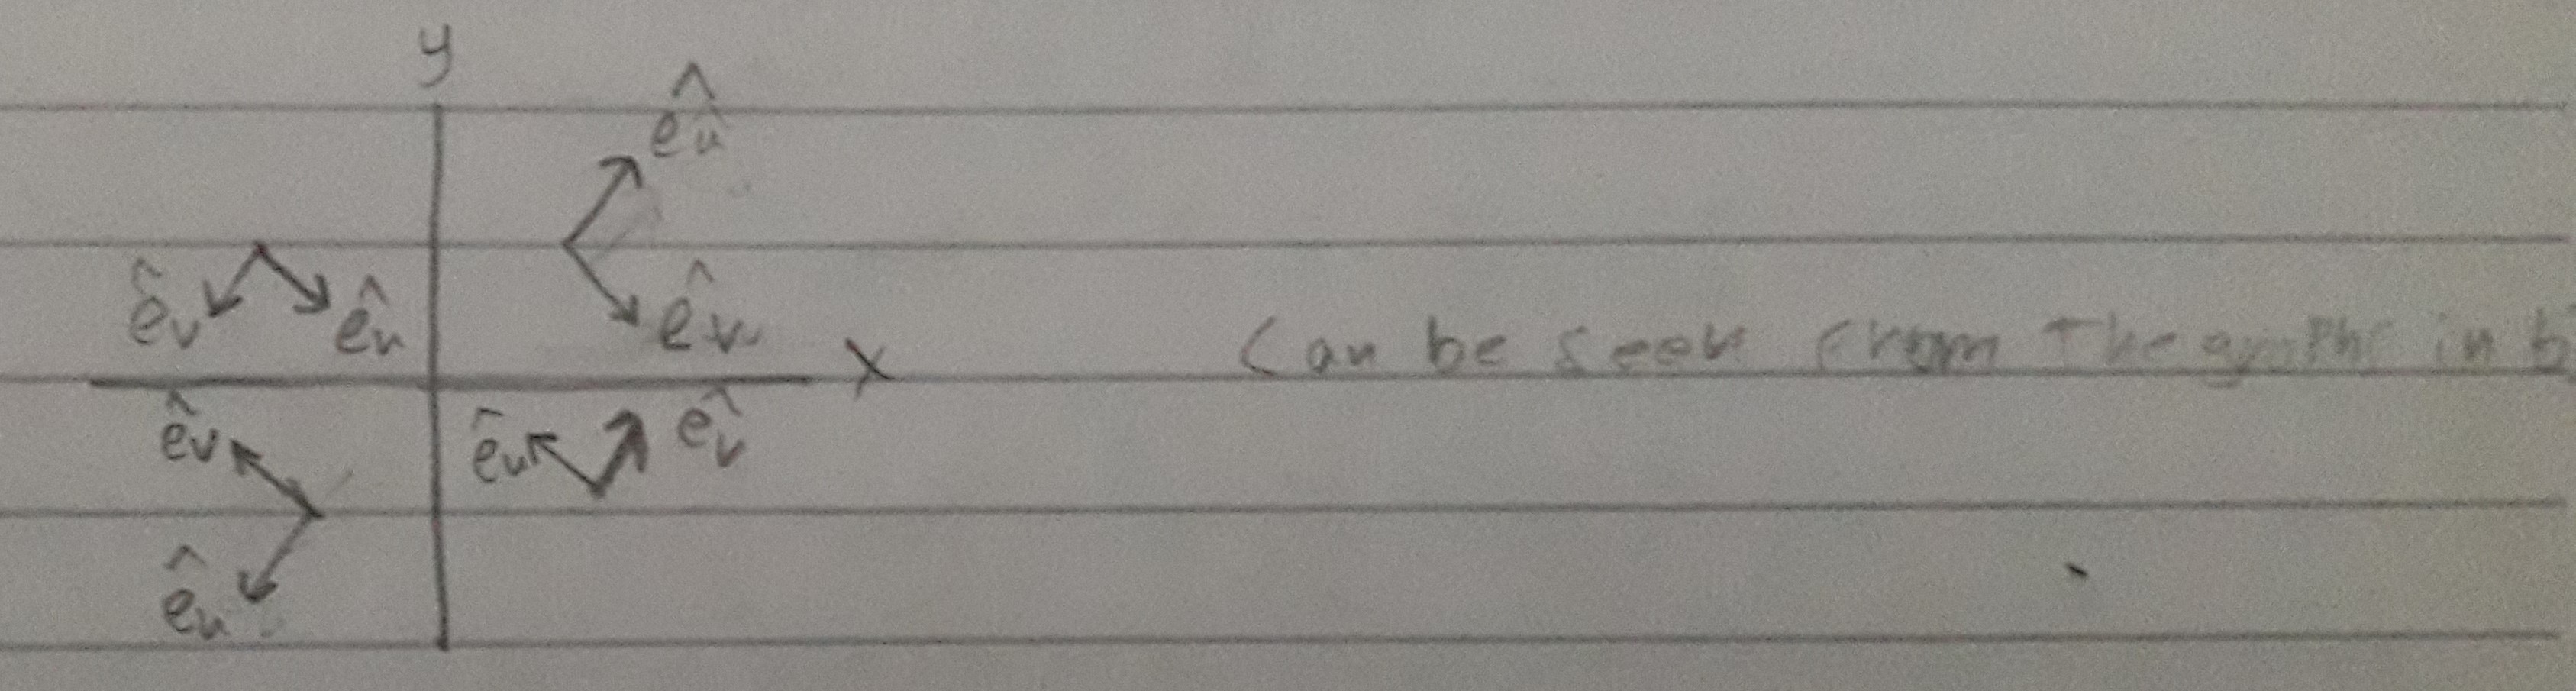
\includegraphics[width=\linewidth]{Q1C.jpg}
    \caption{Basis Vectors Field Plot sketch.}\label{fig:Q1C2}
\end{figure}

\subsubsection{d}

\[
    \hat{\mathbf{e}}_u \times \hat{\mathbf{e}}_v =
    \begin{vmatrix}
        \hat{\dot{\imath}}         & \hat{\dot{\jmath}}          & \hat{k} \\
        \frac{y}{\sqrt{x^2 + y^2}} & \frac{x}{\sqrt{x^2 + y^2}}  & 0       \\
        \frac{x}{\sqrt{x^2 + y^2}} & -\frac{y}{\sqrt{x^2 + y^2}} & 0       \\
    \end{vmatrix}
\]

\[
    = \left(
    - \frac{y}{\sqrt{x^2 + y^2}} \frac{y}{\sqrt{x^2 + y^2}}
    - \frac{x}{\sqrt{x^2 + y^2}} \frac{x}{\sqrt{x^2 + y^2}}
    \right) \hat{k} = -\hat{k}
\]

From the previous result, we can see that the coordinate system is left-handed.

\section{3.10.4}

\subsection{Problem}

With \(\hat{\mathbf{e}}_1\) a unit vector in the direction of increasing \(q_1\), show that
\bigskip

\begin{enumerate}[label= \textbf{(\alph*)}]
    \item
          \(
          \nabla \cdot \hat{\mathbf{e}}_1 =
          \frac{1}{h_1 h_2 h_3} \frac{\partial \left(h_2 h_3\right)}{\partial q_1}
          \)

    \item
          \(
          \nabla \times \hat{\mathbf{e}}_1 = \frac{1}{h_1}
          \left[
              \hat{\mathbf{e}}_2 \frac{1}{h_3} \frac{\partial h_1}{\partial q_3}
              - \hat{\mathbf{e}}_3  \frac{1}{h_2}  \frac{\partial h_1}{\partial q_2}
              \right]
          \)
\end{enumerate}
\bigskip

Note that even though \(\hat{\mathbf{e}}_1\) is a unit vector, its divergence and curl \textbf{do
    not necessarily vanish}.

\subsection{Solution}

\(\hat{\mathbf{e}}_1 = \left\langle1, 0, 0\right\rangle \)

\subsubsection{a}

\[
    \nabla \cdot \textbf{V} = \frac{1}{h_1 h_2 h_3}
    \left[
        \frac{\partial}{\partial q_1}\left(V_1 h_2 h_3\right)
        + \frac{\partial}{\partial q_2}\left(V_2 h_1 h_3\right)
        + \frac{\partial}{\partial q_3}\left(V_3 h_1 h_2\right)
        \right]
\]

\[
    \nabla \cdot \hat{\mathbf{e}}_1 = \frac{1}{h_1 h_2 h_3}
    \left[
        \frac{\partial}{\partial q_1}\left(1 * h_2 h_3\right)
        + \frac{\partial}{\partial q_2}\left(0 * h_1 h_3\right)
        + \frac{\partial}{\partial q_3}\left(0 * h_1 h_2\right)
        \right]
\]

\[
    \nabla \cdot \hat{\mathbf{e}}_1 = \frac{1}{h_1 h_2 h_3} \frac{\partial}{\partial q_1}\left(h_2 h_3\right)
\]

\subsubsection{b}

\[
    \nabla \times \textbf{V} = \frac{1}{h_1 h_2 h_3}
    \begin{vmatrix}
        \hat{\mathbf{e}}_1 h_1        & \hat{\mathbf{e}}_2 h_2        & \hat{\mathbf{e}}_3 h_3        \\
        \frac{\partial}{\partial q_1} & \frac{\partial}{\partial q_2} & \frac{\partial}{\partial q_3} \\
        h_1 V_1                       & h_2 V_2                       & h_3 V_3                       \\
    \end{vmatrix}
\]

\[
    \nabla \times \hat{\mathbf{e}}_1 = \frac{1}{h_1 h_2 h_3}
    \begin{vmatrix}
        \hat{\mathbf{e}}_1 h_1        & \hat{\mathbf{e}}_2 h_2        & \hat{\mathbf{e}}_3 h_3        \\
        \frac{\partial}{\partial q_1} & \frac{\partial}{\partial q_2} & \frac{\partial}{\partial q_3} \\
        h_1*1                         & h_2*0                         & h_3*0                         \\
    \end{vmatrix}
\]

\[
    \nabla \times \hat{\mathbf{e}}_1 = \frac{1}{h_1 h_2 h_3}
    \left(
    \hat{\mathbf{e}}_2 h_2 \frac{\partial h_1}{\partial q_3}
    - \hat{\mathbf{e}}_3 h_3 \frac{\partial h_1}{\partial q_2}
    \right)
\]

\[
    \nabla \times \hat{\mathbf{e}}_1 = \frac{1}{h_1}
    \left[
        \hat{\mathbf{e}}_2 \frac{1}{h_3} \frac{\partial h_1}{\partial q_3}
        - \hat{\mathbf{e}}_3  \frac{1}{h_2}  \frac{\partial h_1}{\partial q_2}
        \right]
\]

\section{3.10.5}

\subsection{Problem}

Show that a set of orthogonal unit vectors \(\hat{\mathbf{e}}_i\) may be defined by

\[
    \hat{\mathbf{e}}_i = \frac{1}{h_i} \frac{\partial \textbf{r}}{\partial q_i}
\]

In particular, show that \(\hat{\mathbf{e}}_i \cdot \hat{\mathbf{e}}_i = 1\)  leads to an expression for
\(h_i\) in agreement with

\[
    h_i^2 = {\left(\frac{\partial x}{\partial q_i}\right)}^2
    + {\left(\frac{\partial y}{\partial q_i}\right)}^2 + {\left(\frac{\partial z}{\partial q_i}\right)}^2
\]

The above equation for \(\hat{\mathbf{e}}_i\) may be taken as a starting point for deriving

\[
    \frac{\partial \hat{\mathbf{e}}_i}{\partial q_j}
    = \hat{\mathbf{e}}_j \frac{1}{h_i} \frac{\partial h_j}{\partial q_i}, \quad i \neq j
\]

\[
    \frac{\partial \hat{\mathbf{e}}_i}{\partial q_i}
    = - \sum_{j \neq i} \hat{\mathbf{e}}_j \frac{1}{h_j} \frac{\partial h_i}{\partial q_j}
\]

\subsection{Solution}

\[
    \hat{\mathbf{e}}_i = \frac{1}{h_i} \frac{\partial \textbf{r}}{\partial q_i}
\]

\[
    \hat{\mathbf{e}}_i \cdot \hat{\mathbf{e}}_j = \frac{1}{h_i h_j}
    \left(\frac{\partial \textbf{r}}{\partial q_i}\right)
    \cdot \left(\frac{\partial \textbf{r}}{\partial q_j}\right)  = \delta_{ij}
\]

\[
    \frac{\partial \textbf{r}}{\partial q_i} = \frac{\partial (x_j \hat{\varepsilon}_j)}{\partial q_i}
    = \frac{\partial x_j}{\partial q_i} \hat{\varepsilon}_j + x_j \frac{\partial \hat{\varepsilon}_j}{\partial q_i}
\]

\[
    \because  \hat{\varepsilon}_{ij} = \delta_{ij}
\]

\[
    \therefore \frac{\partial \hat{\varepsilon}_j}{\partial q_i} = 0
\]

\[
    \frac{\partial \textbf{r}}{\partial q_i} = \frac{\partial x_j}{\partial q_i} \hat{\varepsilon}_j
\]

\[
    \frac{\partial \textbf{r}}{\partial q_i} \cdot \frac{\partial \textbf{r}}{\partial q_j}
    = \frac{\partial x_k}{\partial q_i} \frac{\partial x_m}{\partial q_j}
    \left(\hat{\varepsilon}_k \cdot \hat{\varepsilon}_m\right)
\]

\[
    = \frac{\partial x_k}{\partial q_i} \frac{\partial x_m}{\partial q_j} \delta_{km}
    = \frac{\partial x_k}{\partial q_i} \frac{\partial x_k}{\partial q_j}
\]

\[
    \hat{\mathbf{e}}_i \cdot \hat{\mathbf{e}}_j
    = \frac{1}{h_i h_j} \frac{\partial x_k}{\partial q_i} \frac{\partial x_k}{\partial q_j} = \delta_{ij}
\]

\[
    \frac{\partial x_k}{\partial q_i} \frac{\partial x_k}{\partial q_j} = h_i h_j \delta_{ij}
\]

\[
    i = j \implies {\left(\frac{\partial x_k}{\partial q_i}\right)}^2 = h_i^2
\]

\[
    \because \frac{\partial (h_i \hat{\mathbf{e}}_i)}{\partial q_j}
    = \frac{\partial h_i}{\partial q_j} \hat{\mathbf{e}}_i
    + h_i \frac{\partial \hat{\mathbf{e}}_i}{\partial q_j}
\]

\[
    \because \frac{\partial (h_i \hat{\mathbf{e}}_i)}{\partial q_j}
    = \frac{\partial}{\partial q_j} \left(\frac{\partial \textbf{r}}{\partial q_i}\right)
    = \frac{\partial^2 \textbf{r}}{\partial q_j \partial q_i}
\]

\[
    \because i \neq j \implies \frac{\partial q_i}{\partial q_j} = \frac{\partial q_j}{\partial q_i} = 0
\]

\[
    \therefore \frac{\partial^2 \textbf{r}}{\partial q_j \partial q_i}
    = \frac{\partial^2 \textbf{r}}{\partial q_i \partial q_j}
\]

\[
    = \frac{\partial (h_j \hat{\mathbf{e}}_j)}{\partial q_i}
\]

\[
    \therefore \frac{\partial h_i}{\partial q_j} \hat{\mathbf{e}}_i
    + h_i \frac{\partial \hat{\mathbf{e}}_i}{\partial q_j}
    = \frac{\partial h_j}{\partial q_i} \hat{\mathbf{e}}_j
    + h_j \frac{\partial \hat{\mathbf{e}}_j}{\partial q_i}
\]

\[
    \because \frac{\partial \hat{\mathbf{e}}_i}{\partial q_j} = f\left(q_j\right)  \hat{\mathbf{e}}_j
\]

We can now equate both pairs.

\[
    \therefore\frac{\partial \hat{\mathbf{e}}_i}{\partial q_j}
    = \frac{1}{h_i} \frac{\partial h_j}{\partial q_i} \hat{\mathbf{e}}_j, \quad i \neq j
\]

\[
    \hat{\mathbf{e}}_i \cdot \hat{\mathbf{e}}_j = \delta_{ij} \implies
    \frac{\partial \left(\hat{\mathbf{e}}_i \cdot \hat{\mathbf{e}}_j\right) }{\partial q_k}
    = \hat{\mathbf{e}}_i \cdot \frac{\partial \hat{\mathbf{e}}_j}{\partial q_k}
    +  \frac{\partial \hat{\mathbf{e}}_i}{\partial q_k} \cdot \hat{\mathbf{e}}_j = 0
\]

\[
    \hat{\mathbf{e}}_i \cdot \frac{\partial \hat{\mathbf{e}}_j}{\partial q_k}
    = -\frac{\partial \hat{\mathbf{e}}_i}{\partial q_k} \cdot \hat{\mathbf{e}}_j
\]

We are interested in the case where \(i = k\).

\[
    \hat{\mathbf{e}}_i \cdot \frac{\partial \hat{\mathbf{e}}_j}{\partial q_i}
    = -\frac{\partial \hat{\mathbf{e}}_i}{\partial q_i} \cdot \hat{\mathbf{e}}_j
\]

From this relation, we can derive two statements.

\[
    \hat{\mathbf{e}}_i \cdot \frac{\partial \hat{\mathbf{e}}_i}{\partial q_i} = 0
\]

Which tells us that the change of \(\hat{\mathbf{e}}_i\) in the \(q_i\) direction is
perpendicular to \(\hat{\mathbf{e}}_i\) (if it exists).

\[
    \hat{\mathbf{e}}_j \cdot \frac{\partial \hat{\mathbf{e}}_i}{\partial q_i}
    = - \hat{\mathbf{e}}_i \cdot \frac{\partial \hat{\mathbf{e}}_j}{\partial q_i}, \quad i \neq j
\]

\[
    \hat{\mathbf{e}}_j \cdot \frac{\partial \hat{\mathbf{e}}_i}{\partial q_j}
    = \frac{1}{h_i} \frac{\partial h_j}{\partial q_i} \hat{\mathbf{e}}_j \cdot \hat{\mathbf{e}}_j
\]

\[
    = \frac{1}{h_i} \frac{\partial h_j}{\partial q_i}
\]

\[
    \hat{\mathbf{e}}_j \cdot \frac{\partial \hat{\mathbf{e}}_i}{\partial q_i}
    = - \frac{1}{h_j} \frac{\partial h_i}{\partial q_j}
\]

Now we just add all the components of \(\frac{\partial \hat{\mathbf{e}}_i}{\partial q_i}\)
together to get the final result.

\[
    \frac{\partial \hat{\mathbf{e}}_i}{\partial q_i}
    = - \sum_{j \neq i} \hat{\mathbf{e}}_j \frac{1}{h_j} \frac{\partial h_i}{\partial q_j}
\]

\section{3.10.28}\label{3.10.28}

\subsection{Problem}

Express \(\partial/\partial x, \partial/\partial y, \partial/\partial z\) in spherical polar coordinates.

\bigskip

\textbf{ANS.}
\[
    \frac{\partial}{\partial x} = \sin{\theta} \cos{\varphi} \frac{\partial}{\partial r}
    + \cos{\theta} \cos{\varphi} \frac{1}{r} \frac{\partial}{\partial \theta}
    - \sin{\varphi} \frac{1}{r \sin{\theta}} \frac{\partial}{\partial \varphi}
\]

\[
    \frac{\partial}{\partial y} = \sin{\theta} \sin{\varphi} \frac{\partial}{\partial r}
    + \cos{\theta} \sin{\varphi} \frac{1}{r} \frac{\partial}{\partial \theta}
    + \cos{\varphi} \frac{1}{r \sin{\theta}} \frac{\partial}{\partial \varphi}
\]

\[
    \frac{\partial}{\partial z} = \cos{\theta} \frac{\partial}{\partial r}
    - \sin{\theta} \frac{1}{r} \frac{\partial}{\partial \theta}
\]

\bigskip

\textbf{Hint.} Equate \(\nabla_{xyz}\) and \(\nabla_{r \theta \varphi }\).

\subsection{Solution}

\[
    x = r \sin{\theta} \cos{\varphi}, y = r \sin{\theta} \sin{\varphi}, z = r \cos{\theta}
\]

\[
    \nabla = \hat{\mathbf{e}}_1 \frac{1}{h_1} \frac{\partial}{\partial q_1}
    + \hat{\mathbf{e}}_2 \frac{1}{h_2} \frac{\partial}{\partial q_2}
    + \hat{\mathbf{e}}_3 \frac{1}{h_3} \frac{\partial}{\partial q_3}
\]

\[
    \nabla_{xyz} =  \hat{\dot{\imath}} \frac{\partial}{\partial x}
    + \hat{\dot{\jmath}} \frac{\partial}{\partial y}
    +  \hat{k} \frac{\partial}{\partial z}
\]

\[
    \nabla_{r \theta \varphi } = \hat{\mathbf{e}}_r \frac{\partial}{\partial r}
    + \hat{\mathbf{e}}_\theta \frac{1}{r} \frac{\partial}{\partial \theta}
    + \hat{\mathbf{e}}_\varphi \frac{1}{r \sin{\theta}} \frac{\partial}{\partial \varphi}
\]

\[
    \nabla_{xyz} = \nabla_{r \theta \varphi }
\]

\[
    \hat{\dot{\imath}} \frac{\partial}{\partial x}
    + \hat{\dot{\jmath}} \frac{\partial}{\partial y}
    +  \hat{k} \frac{\partial}{\partial z} = \hat{\mathbf{e}}_r \frac{\partial}{\partial r}
    + \hat{\mathbf{e}}_\theta \frac{1}{r} \frac{\partial}{\partial \theta}
    + \hat{\mathbf{e}}_\varphi \frac{1}{r \sin{\theta}} \frac{\partial}{\partial \varphi}
\]

\[
    \hat{\mathbf{e}}_r = \frac{\partial x_j}{\partial r} \hat{\varepsilon}_j
    + x_j \frac{\partial \hat{\varepsilon}_j}{\partial r} = \frac{\partial x}{\partial r} \hat{\dot{\imath}}
    + \frac{\partial y}{\partial r} \hat{\dot{\jmath}} + \frac{\partial z}{\partial r} \hat{k}
\]

\[
    = \sin{\theta} \cos{\varphi} \hat{\dot{\imath}} + \sin{\theta} \sin{\varphi} \hat{\dot{\jmath}}
    + \cos{\theta} \hat{k}
\]

\[
    \hat{\mathbf{e}}_\theta = \cos{\theta} \cos{\varphi} \hat{\dot{\imath}}
    + \cos{\theta} \sin{\varphi} \hat{\dot{\jmath}} - \sin{\theta} \hat{k}
\]

\[
    \hat{\mathbf{e}}_\varphi = -\sin{\varphi} \hat{\dot{\imath}} + \cos{\varphi} \hat{\dot{\jmath}}
\]

\[
    \hat{\dot{\imath}} \frac{\partial}{\partial x} + \hat{\dot{\jmath}} \frac{\partial}{\partial y}
    +  \hat{k} \frac{\partial}{\partial z} =
    \left(
    \sin{\theta} \cos{\varphi} \hat{\dot{\imath}}
    + \sin{\theta} \sin{\varphi} \hat{\dot{\jmath}}
    + \cos{\theta} \hat{k}
    \right)  \frac{\partial}{\partial r}
\]

\[
    + \left(
    \cos{\theta} \cos{\varphi} \hat{\dot{\imath}} + \cos{\theta} \sin{\varphi} \hat{\dot{\jmath}}
    - \sin{\theta} \hat{k}
    \right) \frac{1}{r} \frac{\partial}{\partial \theta}
\]

\[
    + \left(-\sin{\varphi} \hat{\dot{\imath}} + \cos{\varphi} \hat{\dot{\jmath}}\right)
    \frac{1}{r \sin{\theta}} \frac{\partial}{\partial \varphi}
\]

\[
    = \hat{\dot{\imath}}
    \left(
    \sin{\theta} \cos{\varphi} \frac{\partial}{\partial r}
    + \cos{\theta} \cos{\varphi} \frac{1}{r} \frac{\partial}{\partial \theta}
    - \sin{\varphi} \frac{1}{r \sin{\theta}} \frac{\partial}{\partial \varphi}
    \right)
\]

\[
    + \hat{\dot{\jmath}}
    \left(
    \sin{\theta} \sin{\varphi} \frac{\partial}{\partial r}
    + \cos{\theta} \sin{\varphi} \frac{1}{r} \frac{\partial}{\partial \theta}
    + \cos{\varphi} \frac{1}{r \sin{\theta}} \frac{\partial}{\partial \varphi}
    \right)
\]

\[
    + \hat{k} \left(\cos{\theta} \frac{\partial}{\partial r}
    - \sin{\theta} \frac{1}{r} \frac{\partial}{\partial \theta} \right)
\]

\[
    \frac{\partial}{\partial x} = \sin{\theta} \cos{\varphi} \frac{\partial}{\partial r}
    + \cos{\theta} \cos{\varphi} \frac{1}{r} \frac{\partial}{\partial \theta}
    - \sin{\varphi} \frac{1}{r \sin{\theta}} \frac{\partial}{\partial \varphi}
\]

\[
    \frac{\partial}{\partial y} = \sin{\theta} \sin{\varphi} \frac{\partial}{\partial r}
    + \cos{\theta} \sin{\varphi} \frac{1}{r} \frac{\partial}{\partial \theta}
    + \cos{\varphi} \frac{1}{r \sin{\theta}} \frac{\partial}{\partial \varphi}
\]

\[
    \frac{\partial}{\partial z} = \cos{\theta} \frac{\partial}{\partial r}
    - \sin{\theta} \frac{1}{r} \frac{\partial}{\partial \theta}
\]

\section{3.10.29}

\subsection{Problem}

Using results from \hyperref[3.10.28]{Exercise 3.10.28}, show that

\[
    -i \left(x \frac{\partial}{\partial y} - y \frac{\partial}{\partial x}\right)
    = - i \frac{\partial}{\partial \varphi}
\]

This is the quantum mechanical operator corresponding to the \(z-\)component of orbital
angular momentum.

\subsection{Solution}

\[
    x = r \sin{\theta} \cos{\varphi}, y = r \sin{\theta} \sin{\varphi}
\]

\[
    -i \left(x \frac{\partial}{\partial y} - y \frac{\partial}{\partial x}\right)
\]

\[
    =
    -i r \sin{\theta} \cos{\varphi}
    \left(
    \sin{\theta} \sin{\varphi} \frac{\partial}{\partial r}
    + \cos{\theta} \sin{\varphi} \frac{1}{r} \frac{\partial}{\partial \theta}
    + \cos{\varphi} \frac{1}{r \sin{\theta}} \frac{\partial}{\partial \varphi}
    \right)
\]

\[
    + i r \sin{\theta} \sin{\varphi}
    \left(
    \sin{\theta} \cos{\varphi} \frac{\partial}{\partial r}
    + \cos{\theta} \cos{\varphi} \frac{1}{r} \frac{\partial}{\partial \theta}
    - \sin{\varphi} \frac{1}{r \sin{\theta}} \frac{\partial}{\partial \varphi}
    \right)
\]

\[
    = i r \sin{\theta}
    \left(\sin{\theta} \sin{\varphi} \cos{\varphi} - \sin{\theta} \sin{\varphi} \cos{\varphi} \right)
    \frac{\partial}{\partial r}
\]

\[
    + i r \sin{\theta}
    \left(\sin{\varphi} \cos{\varphi} - \sin{\varphi} \cos{\varphi}\right)
    \cos{\theta} \frac{1}{r} \frac{\partial}{\partial \theta}
\]

\[
    - i \left(\sin^2{\varphi} + \cos^2{\varphi} \right) \frac{\partial}{\partial \varphi}
\]

\[
    = - i \frac{\partial}{\partial \varphi}
\]

\section{3.10.30}

\subsection{Problem}

With the quantum mechanical orbital angular momentum operator defined as
\(\textbf{L} = -i \left(\textbf{r} \times \nabla\right)\), show that
\bigskip

\begin{enumerate}[label= \textbf{(\alph*)}]
    \item
          \(
          L_x + i L_y = e^{i \varphi}
          \left(
          \frac{\partial}{\partial \theta}
          + i \cot{\theta}\frac{\partial}{\partial \varphi}
          \right)
          \)

    \item
          \(
          L_x - i L_y = - e^{- i \varphi}
          \left(
          \frac{\partial}{\partial \theta}
          - i \cot{\theta}\frac{\partial}{\partial \varphi}
          \right)
          \)
\end{enumerate}
\bigskip

\subsection{Solution}

\[
    \textbf{L} = -i \left(\textbf{r} \times \nabla\right)
\]

\[
    = -i \left\lvert \begin{array}{ccc}
        \hat{\dot{\imath}}          & \hat{\dot{\jmath}}          & \hat{k}                     \\
        x                           & y                           & z                           \\
        \frac{\partial}{\partial x} & \frac{\partial}{\partial y} & \frac{\partial}{\partial z} \\
    \end{array} \right\rvert
\]

\[
    =
    -i
    \left(
    \hat{\dot{\imath}} \left(y \frac{\partial}{\partial z} - z \frac{\partial}{\partial y}\right)
    + \hat{\dot{\jmath}} \left(z \frac{\partial}{\partial x} - x \frac{\partial}{\partial z}\right)
    + \hat{k} \left(x \frac{\partial}{\partial y} - y \frac{\partial}{\partial x}\right)
    \right)
\]

\[
    = i \left(z \frac{\partial}{\partial y} - y \frac{\partial}{\partial z}\right) \hat{\dot{\imath}}
    + i \left(x \frac{\partial}{\partial z} - z \frac{\partial}{\partial x}\right) \hat{\dot{\jmath}}
    + i \left(y \frac{\partial}{\partial x} - x \frac{\partial}{\partial y}\right) \hat{k}
\]

\[
    L_x = i \left(z \frac{\partial}{\partial y} - y \frac{\partial}{\partial z}\right)
\]

\[
    L_y = i \left(x \frac{\partial}{\partial z} - z \frac{\partial}{\partial x}\right)
\]

\[
    L_z = i \left(y \frac{\partial}{\partial x} - x \frac{\partial}{\partial y}\right)
\]

\subsubsection{a}

\[
    L_x + i L_y = i \left(z \frac{\partial}{\partial y} - y \frac{\partial}{\partial z}\right)
    - \left(x \frac{\partial}{\partial z} - z \frac{\partial}{\partial x}\right)
\]

\[
    = z \frac{\partial}{\partial x} + i z \frac{\partial}{\partial y} - \left(x + i y\right)
    \frac{\partial}{\partial z}
\]

\[
    = z \left(\frac{\partial}{\partial x} + i \frac{\partial}{\partial y}\right)  - \left(x + i y\right)
    \frac{\partial}{\partial z}
\]

\[
    x + i y = r \sin{\theta} \cos{\varphi} + i r \sin{\theta} \sin{\varphi} = r \sin{\theta}
    \left(\cos{\varphi} + i \sin{\varphi}\right) = r \sin{\theta} e^{i \varphi}
\]

\[
    \frac{\partial}{\partial x} + i \frac{\partial}{\partial y} =
\]

\[
    \sin{\theta} \cos{\varphi} \frac{\partial}{\partial r}
    + \cos{\theta} \cos{\varphi} \frac{1}{r} \frac{\partial}{\partial \theta}
    - \sin{\varphi} \frac{1}{r \sin{\theta}} \frac{\partial}{\partial \varphi}
\]

\[
    + i  \sin{\theta} \sin{\varphi} \frac{\partial}{\partial r}
    + i \cos{\theta} \sin{\varphi} \frac{1}{r} \frac{\partial}{\partial \theta}
    + i \cos{\varphi} \frac{1}{r \sin{\theta}} \frac{\partial}{\partial \varphi}
\]

\[
    = \sin{\theta} \left(\cos{\varphi} + i \sin{\varphi}\right) \frac{\partial}{\partial r}
    + \cos{\theta} \left(\cos{\varphi} + i \sin{\varphi}\right) \frac{1}{r} \frac{\partial}{\partial \theta}
\]

\[
    + \left(i \cos{\varphi} - \sin{\varphi}\right)  \frac{1}{r \sin{\theta}} \frac{\partial}{\partial \varphi}
\]

\[
    = e^{i \varphi}
    \left(
    \sin{\theta} \frac{\partial}{\partial r}+ \cos{\theta} \frac{1}{r} \frac{\partial}{\partial \theta}
    + i \frac{1}{r \sin{\theta}} \frac{\partial}{\partial \varphi}
    \right)
\]

\[
    L_x + i L_y =
\]

\[
    r \cos{\theta} e^{i \varphi}
    \left(
    \sin{\theta} \frac{\partial}{\partial r}
    + \cos{\theta} \frac{1}{r} \frac{\partial}{\partial \theta}
    + i \frac{1}{r \sin{\theta}} \frac{\partial}{\partial \varphi}
    \right)
\]

\[
    - r \sin{\theta} e^{i \varphi}
    \left(
    \cos{\theta} \frac{\partial}{\partial r} - \sin{\theta} \frac{1}{r} \frac{\partial}{\partial \theta}
    \right)
\]

\[
    = r e^{i \varphi}
    \left(
    \sin{\theta} \cos{\theta} \frac{\partial}{\partial r}
    + \frac{\cos^2{\theta}}{r} \frac{\partial}{\partial \theta}
    + i \cot{\theta} \frac{1}{r}\frac{\partial}{\partial \varphi}
    - \sin{\theta} \cos{\theta} \frac{\partial}{\partial r}
    + \frac{\sin^2{\theta}}{r} \frac{\partial}{\partial \theta}
    \right)
\]

\[
    = e^{i \varphi}
    \left(
    \frac{\partial}{\partial \theta}
    + i \cot{\theta}\frac{\partial}{\partial \varphi}
    \right)
\]

\subsubsection{b}

\[
    L_x - i L_y = i \left(z \frac{\partial}{\partial y} - y \frac{\partial}{\partial z}\right)
    + \left(x \frac{\partial}{\partial z} - z \frac{\partial}{\partial x}\right)
\]

\[
    = z \left(i \frac{\partial}{\partial y} - \frac{\partial}{\partial x}\right) + \left( x - i y\right)
    \frac{\partial}{\partial z}
\]

\[
    x - i y = r \sin{\theta} \cos{\varphi} - i r \sin{\theta} \sin{\varphi} = r \sin{\theta}
    \left(\cos{\varphi} - i \sin{\varphi}\right) = r \sin{\theta} e^{-i \varphi}
\]

\[
    i \frac{\partial}{\partial y} - \frac{\partial}{\partial x} =
\]

\[
    i  \sin{\theta} \sin{\varphi} \frac{\partial}{\partial r}
    + i \cos{\theta} \sin{\varphi} \frac{1}{r} \frac{\partial}{\partial \theta}
    + i \cos{\varphi} \frac{1}{r \sin{\theta}} \frac{\partial}{\partial \varphi}
\]

\[
    - \sin{\theta} \cos{\varphi} \frac{\partial}{\partial r}
    - \cos{\theta} \cos{\varphi} \frac{1}{r} \frac{\partial}{\partial \theta}
    + \sin{\varphi} \frac{1}{r \sin{\theta}} \frac{\partial}{\partial \varphi}
\]

\[
    = -\sin{\theta} \left(\cos{\varphi} - i \sin{\varphi}\right) \frac{\partial}{\partial r}
    - \cos{\theta} \left(\cos{\varphi} - i \sin{\varphi}\right) \frac{1}{r} \frac{\partial}{\partial \theta}
\]

\[
    + i \left(\cos{\varphi} - i \sin{\varphi}\right) \frac{1}{r \sin{\theta}} \frac{\partial}{\partial \varphi}
\]

\[
    = - e^{-i \varphi}
    \left(
    \sin{\theta} \frac{\partial}{\partial r}
    + \cos{\theta} \frac{1}{r} \frac{\partial}{\partial \theta}
    + i \frac{1}{r \sin{\theta}} \frac{\partial}{\partial \varphi}
    \right)
\]

\[
    L_x - i L_y =
\]

\[
    - r \cos{\theta} e^{-i \varphi}
    \left(
    \sin{\theta} \frac{\partial}{\partial r}
    + \cos{\theta} \frac{1}{r} \frac{\partial}{\partial \theta}
    + i \frac{1}{r \sin{\theta}} \frac{\partial}{\partial \varphi}
    \right)
\]

\[
    + r \sin{\theta} e^{-i \varphi}
    \left(
    \cos{\theta} \frac{\partial}{\partial r} - \sin{\theta} \frac{1}{r} \frac{\partial}{\partial \theta}
    \right)
\]

\[
    = - r e^{-i \varphi}
    \left(
    \sin{\theta} \cos{\theta} \frac{\partial}{\partial r}
    + \frac{\cos^2{\theta}}{r} \frac{\partial}{\partial \theta}
    + i \frac{\cot{\theta}}{r}\frac{\partial}{\partial \varphi}
    - \sin{\theta} \cos{\theta} \frac{\partial}{\partial r}
    + \frac{\sin^2{\theta}}{r} \frac{\partial}{\partial \theta}
    \right)
\]

\[
    = - e^{-i \varphi}
    \left(
    \frac{\partial}{\partial \theta}
    - i \cot{\theta}\frac{\partial}{\partial \varphi}
    \right)
\]

\section{3.10.31}

\subsection{Problem}

Verify that \(\textbf{L} \times \textbf{L} = i \textbf{L}\) in spherical polar coordinates.
\(\textbf{L} = -i \left(\textbf{r} \times \nabla\right)\), the quantum mechanical orbital angular
momentum operator.

Written in component form, this relation is

\[
    L_y L_z - L_z L_y = i L_x , \quad L_z L_x - L_x L_z = i L_y ,\quad L_x L_y - L_y L_x = i L_z
\]

Using the commutator notation, \([A, B] = AB - BA\), and the definition of the Levi-Civita symbol
\(\varepsilon_{ijk}\), the above can also be written

\[
    [L_i, L_j] = i \varepsilon_{ijk} L_k
\]

where \(i , j , k\) are \(x, y, z\) in any order.

\textbf{Hint.} Use spherical polar coordinates for \textbf{L}
but Cartesian components for the cross product.

\subsection{Solution}

\[
    \textbf{L} = -i \left(\textbf{r} \times \nabla\right)
    = i
    \left(
    \hat{\mathbf{e}}_\theta \frac{1}{\sin{\theta}} \frac{\partial}{\partial \varphi}
    - \hat{\mathbf{e}}_\varphi \frac{\partial}{\partial \theta}
    \right)
\]

\[
    \hat{\mathbf{e}}_r
    = \sin{\theta} \cos{\varphi} \hat{\dot{\imath}} + \sin{\theta} \sin{\varphi} \hat{\dot{\jmath}}
    + \cos{\theta} \hat{k}
\]

\[
    \hat{\mathbf{e}}_\theta
    = \cos{\theta} \cos{\varphi} \hat{\dot{\imath}}
    + \cos{\theta} \sin{\varphi} \hat{\dot{\jmath}}
    - \sin{\theta} \hat{k}
\]

\[
    \hat{\mathbf{e}}_\varphi
    = -\sin{\varphi} \hat{\dot{\imath}}
    + \cos{\varphi} \hat{\dot{\jmath}}
\]

\[
    \textbf{J}_{ij} = \frac{\partial \hat{\mathbf{e}}_i}{\partial \hat{\mathbf{e}}_j}
\]

\[
    \left(
    \begin{array}{ccc}
            \frac{\partial \hat{\mathbf{e}}_\theta}{\partial \theta}  & \frac{\partial \hat{\mathbf{e}}_\theta}{\partial \varphi}  \\
            \frac{\partial \hat{\mathbf{e}}_\varphi}{\partial \theta} & \frac{\partial \hat{\mathbf{e}}_\varphi}{\partial \varphi}
        \end{array}
    \right)
    = \left(
    \begin{array}{ccc}
            - \hat{\mathbf{e}}_r & \cos{\theta} \hat{\mathbf{e}}_\varphi                                  \\
            0                    & - \sin \theta \hat{\mathbf{e}}_r - \cos \theta \hat{\mathbf{e}}_\theta
        \end{array}
    \right)
\]

\[
    \textbf{L} \times \textbf{L} =
    \left(
    \hat{\mathbf{e}}_\theta \frac{1}{\sin{\theta}} \frac{\partial}{\partial \varphi}
    - \hat{\mathbf{e}}_\varphi \frac{\partial}{\partial \theta}
    \right) \times
    \left(
    \hat{\mathbf{e}}_\varphi \frac{\partial}{\partial \theta}
    - \hat{\mathbf{e}}_\theta \frac{1}{\sin{\theta}} \frac{\partial}{\partial \varphi}
    \right)
\]

\[
    = \hat{\mathbf{e}}_\theta \frac{1}{\sin{\theta}} \frac{\partial}{\partial \varphi}
    \times \hat{\mathbf{e}}_\varphi \frac{\partial}{\partial \theta}
    - \hat{\mathbf{e}}_\theta \frac{1}{\sin{\theta}} \frac{\partial}{\partial \varphi}
    \times \hat{\mathbf{e}}_\theta \frac{1}{\sin{\theta}} \frac{\partial}{\partial \varphi}
\]

\[
    - \hat{\mathbf{e}}_\varphi \frac{\partial}{\partial \theta}
    \times \hat{\mathbf{e}_\varphi} \frac{\partial}{\partial \theta}
    + \hat{\mathbf{e}}_\varphi \frac{\partial}{\partial \theta}
    \times \hat{\mathbf{e}}_\theta \frac{1}{\sin{\theta}} \frac{\partial}{\partial \varphi}
\]

\[
    =\left(\hat{\mathbf{e}}_\theta \times \frac{\partial \hat{\mathbf{e}}_\varphi}{\partial \varphi}\right)
    \frac{1}{\sin{\theta}} \frac{\partial}{\partial \theta}
    + \cancel{\left(\hat{\mathbf{e}}_\theta \times \hat{\mathbf{e}}_\varphi\right)
        \frac{1}{\sin{\theta}} \frac{\partial^2}{\partial \varphi \partial \theta}}
\]

\[
    - \left(\hat{\mathbf{e}}_\varphi \times \frac{\partial \hat{\mathbf{e}}_\theta}{\partial \varphi}\right)
    \frac{1}{\sin^2{\theta}} \frac{\partial}{\partial \varphi}
    - \cancelto{0}{\left(\hat{\mathbf{e}}_\theta \times \hat{\mathbf{e}}_\theta\right)
    \frac{1}{\sin^2{\theta}} \frac{\partial^2}{\partial \varphi^2}}
\]

\[
    - \cancelto{0}{\left(\hat{\mathbf{e}}_\varphi \times \frac{\partial \hat{\mathbf{e}}_\varphi}{\partial \theta}\right)
        \frac{\partial}{\partial \theta}}
    - \cancelto{0}{\left(\hat{\mathbf{e}}_\varphi \times \hat{\mathbf{e}}_\varphi\right)
        \frac{\partial^2}{\partial \theta^2}}
\]

\[
    + \left(\hat{\mathbf{e}}_\varphi \times \frac{\partial \hat{\mathbf{e}}_\theta}{\partial \theta}\right)
    \frac{1}{\sin{\theta}} \frac{\partial}{\partial \varphi}
    + \cancel{\left(\hat{\mathbf{e}}_\varphi \times \hat{\mathbf{e}}_\theta\right)
        \frac{1}{\sin{\theta}} \frac{\partial^2}{\partial \theta \partial \varphi}}
\]

\[
    = - \left(
    \hat{\mathbf{e}}_\theta \times \left(\sin \theta \hat{\mathbf{e}}_r + \cos \theta \hat{\mathbf{e}}_\theta\right)
    \right)
    \frac{1}{\sin{\theta}} \frac{\partial}{\partial \theta}
\]

\[
    - \cancelto{0}{\left(\hat{\mathbf{e}}_\varphi \times \hat{\mathbf{e}}_\varphi\right)
    \frac{\cos{\theta}}{\sin^2{\theta}} \frac{\partial}{\partial \varphi}}
\]

\[
    - \left(\hat{\mathbf{e}}_\varphi \times \hat{\mathbf{e}}_r\right)
    \frac{1}{\sin{\theta}} \frac{\partial}{\partial \varphi}
\]

\[
    = - \left(\hat{\mathbf{e}}_\theta \times \hat{\mathbf{e}}_r\right)
    \frac{\partial}{\partial \theta}
    + \cancelto{0}{\left(\hat{\mathbf{e}}_\theta \times \hat{\mathbf{e}}_\theta\right)
    \cot{\theta} \frac{\partial}{\partial \theta}}
    - \left(\hat{\mathbf{e}}_\varphi \times \hat{\mathbf{e}}_r\right)
    \frac{1}{\sin{\theta}} \frac{\partial}{\partial \varphi}
\]

\[
    = \hat{\mathbf{e}}_\varphi \frac{\partial}{\partial \theta}
    - \hat{\mathbf{e}}_\theta \frac{1}{\sin{\theta}} \frac{\partial}{\partial \varphi}
\]

\[
  = i \textbf{L}   
\]

\section{3.10.32}

\subsection{Problem}

\begin{enumerate}[label= \textbf{(\alph*)}]
    \item Using
          \[
              \nabla \psi (r, \theta, \varphi) = \hat{\mathbf{e}}_r \frac{\partial \psi}{\partial r}
              + \hat{\mathbf{e}}_\theta \frac{1}{r} \frac{\partial \psi}{\partial \theta}
              + \hat{\mathbf{e}}_\varphi \frac{1}{r \sin{\theta}} \frac{\partial \psi}{\partial \varphi}
          \]

          show that

          \[
              \textbf{L} = -i \left(\textbf{r} \times \nabla\right)
              = i
              \left(
              \hat{\mathbf{e}}_\theta \frac{1}{\sin{\theta}} \frac{\partial}{\partial \varphi}
              - \hat{\mathbf{e}}_\varphi \frac{\partial}{\partial \theta}
              \right)
          \]

    \item Resolving \(\hat{\mathbf{e}}_\theta \) and \(\hat{\mathbf{e}}_\varphi \)
          into Cartesian components, determine \(L_x, L_y\), and \(L_z\) in terms of
          \(\theta , \varphi \), and their derivatives.

    \item From \(L^2 = L_x^2 + L_y^2 + L_z^2\) show that
          \[
              \textbf{L}^2 = -\frac{1}{\sin{\theta}} \frac{\partial}{\partial \theta}
              \left(\sin{\theta} \frac{\partial}{\partial \theta}\right)
              - \frac{1}{\sin^2{\theta}} \frac{\partial^2}{\partial \varphi^2}
          \]

          \[
              = -r^2 \nabla^2 + \frac{\partial}{\partial r} \left(r^2 \frac{\partial}{\partial r}\right)
          \]
\end{enumerate}

\subsection{Solution}

\subsubsection{a}

\[
    \textbf{L} = -i \left(\textbf{r} \times \nabla\right)
\]

\[
    \textbf{r} = r \hat{\mathbf{e}}_r
\]

\[
    \nabla_{r \theta \varphi } = \hat{\mathbf{e}}_r \frac{\partial}{\partial r}
    + \hat{\mathbf{e}}_\theta \frac{1}{r} \frac{\partial}{\partial \theta}
    + \hat{\mathbf{e}}_\varphi \frac{1}{r \sin{\theta}} \frac{\partial}{\partial \varphi}
\]

\[
    \textbf{L} = -i
    \textbf{r} \times
    \left(
    \hat{\mathbf{e}}_r \frac{\partial}{\partial r}
    + \hat{\mathbf{e}}_\theta \frac{1}{r} \frac{\partial}{\partial \theta}
    + \hat{\mathbf{e}}_\varphi \frac{1}{r \sin{\theta}} \frac{\partial}{\partial \varphi}
    \right)
\]

\[
    = -i r
    \left(
    \left(\hat{\mathbf{e}}_r \times \hat{\mathbf{e}}_r\right)  \frac{\partial}{\partial r}
    + \left(\hat{\mathbf{e}}_r \times \hat{\mathbf{e}}_\theta\right)
    \frac{1}{r} \frac{\partial}{\partial \theta}
    + \left(\hat{\mathbf{e}}_r \times \hat{\mathbf{e}}_\varphi\right)
    \frac{1}{r \sin{\theta}} \frac{\partial}{\partial \varphi}
    \right)
\]

\(\because \) spherical polar coordinates are right-handed and orthonormal system.

\[
    \therefore \hat{\mathbf{e}}_i \times \hat{\mathbf{e}}_j = \varepsilon_{ijk} \hat{\mathbf{e}}_k
\]

where \(\varepsilon_{ijk}\) is the Levi-Civita symbol.
\(\varepsilon_{ijk} = 1\) if \(i, j, k\) is an even permutation of \(r, \theta, \varphi \), \(-1\) if it
is an odd permutation, and 0 if any two indices are equal.

\[
    \therefore \textbf{L} = -i r
    \left(
    0  \frac{\partial}{\partial r}
    + 1 \hat{\mathbf{e}}_\varphi
    \frac{1}{r} \frac{\partial}{\partial \theta}
    - 1 \hat{\mathbf{e}}_\theta
    \frac{1}{r \sin{\theta}} \frac{\partial}{\partial \varphi}
    \right)
\]

\[
    = i
    \left(
    \hat{\mathbf{e}}_\theta \frac{1}{\sin{\theta}} \frac{\partial}{\partial \varphi}
    - \hat{\mathbf{e}}_\varphi \frac{\partial}{\partial \theta}
    \right)
\]

\subsubsection{b}

\[
    \hat{\mathbf{e}}_\theta
    = \cos{\theta} \cos{\varphi} \hat{\dot{\imath}}
    + \cos{\theta} \sin{\varphi} \hat{\dot{\jmath}}
    - \sin{\theta} \hat{k}
\]

\[
    \hat{\mathbf{e}}_\varphi
    = -\sin{\varphi} \hat{\dot{\imath}}
    + \cos{\varphi} \hat{\dot{\jmath}}
\]

\[
    \textbf{L} =
    i \left(
    \cos{\theta} \cos{\varphi} \hat{\dot{\imath}}
    + \cos{\theta} \sin{\varphi} \hat{\dot{\jmath}}
    - \sin{\theta} \hat{k}
    \right)
    \frac{1}{\sin{\theta}} \frac{\partial}{\partial \varphi}
    +i \left(
    \sin{\varphi} \hat{\dot{\imath}}
    -\cos{\varphi} \hat{\dot{\jmath}}
    \right)
    \frac{\partial}{\partial \theta}
\]

\[
    = i \cos{\varphi} \cot{\theta} \hat{\dot{\imath}} \frac{\partial}{\partial \varphi}
    + i \sin{\varphi} \cot{\theta} \hat{\dot{\jmath}} \frac{\partial}{\partial \varphi}
    - i \hat{k} \frac{\partial}{\partial \varphi}
    + i \sin{\varphi} \hat{\dot{\imath}} \frac{\partial}{\partial \theta}
    - i \cos{\varphi} \hat{\dot{\jmath}} \frac{\partial}{\partial \theta}
\]

\[
    = - i \hat{\dot{\imath}}
    \left(
    -\cos{\varphi} \cot{\theta}\frac{\partial}{\partial \varphi}
    - \sin{\varphi} \frac{\partial}{\partial \theta}
    \right)
\]

\[
    - i \hat{\dot{\jmath}}
    \left(
    \cos{\varphi} \frac{\partial}{\partial \theta}
    -\sin{\varphi} \cot{\theta}\frac{\partial}{\partial \varphi}
    \right)
    - i \hat{k} \frac{\partial}{\partial \varphi}
\]

\[
    L_x = i
    \left(
    \cos{\varphi} \cot{\theta}\frac{\partial}{\partial \varphi}
    + \sin{\varphi} \frac{\partial}{\partial \theta}
    \right)
\]

\[
    L_y = i
    \left(
    \sin{\varphi} \cot{\theta}\frac{\partial}{\partial \varphi}
    -\cos{\varphi} \frac{\partial}{\partial \theta}
    \right)
\]

\[
    L_z = - i \frac{\partial}{\partial \varphi}
\]

\subsubsection{c}

\[
    L_x^2 =
    -{\left(
    \cos{\varphi} \cot{\theta}\frac{\partial}{\partial \varphi}
    + \sin{\varphi} \frac{\partial}{\partial \theta}
    \right)}^2
\]

\[
    = - \cot^2{\theta} \cos{\varphi} \frac{\partial}{\partial \varphi}
    \left(\cos{\varphi} \frac{\partial}{\partial \varphi}\right)
    - \sin^2{\varphi} \frac{\partial^2}{\partial \theta^2}
\]

\[
    - \cos{\varphi} \cot{\theta}\frac{\partial}{\partial \varphi}
    \left(\sin{\varphi} \frac{\partial}{\partial \theta}\right)
    - \sin{\varphi} \cos{\varphi} \frac{\partial}{\partial \theta}
    \left(\cot{\theta}\frac{\partial}{\partial \varphi}\right)
\]

\[
    L_y^2 =
    -{\left(
    \sin{\varphi} \cot{\theta}\frac{\partial}{\partial \varphi}
    - \cos{\varphi} \frac{\partial}{\partial \theta}
    \right)}^2
\]

\[
    = - \cot^2{\theta} \sin{\varphi} \frac{\partial}{\partial \varphi}
    \left(\sin{\varphi} \frac{\partial}{\partial \varphi}\right)
    - \cos^2{\varphi} \frac{\partial^2}{\partial \theta^2}
\]

\[
    + \sin{\varphi} \cot{\theta}\frac{\partial}{\partial \varphi}
    \left(\cos{\varphi} \frac{\partial}{\partial \theta}\right)
    + \sin{\varphi} \cos{\varphi} \frac{\partial}{\partial \theta}
    \left(\cot{\theta} \frac{\partial}{\partial \varphi}\right)
\]

\[
    L_z^2 = - \frac{\partial^2}{\partial \varphi^2}
\]

\[
    \textbf{L}^2 = L_x^2 + L_y^2 + L_z^2
\]

\[
    = - \cot^2{\theta} \cos{\varphi} \frac{\partial}{\partial \varphi}
    \left(\cos{\varphi} \frac{\partial}{\partial \varphi}\right)
    - \sin^2{\varphi} \frac{\partial^2}{\partial \theta^2}
\]

\[
    - \cos{\varphi} \cot{\theta}\frac{\partial}{\partial \varphi}
    \left(\sin{\varphi} \frac{\partial}{\partial \theta}\right)
    - \sin{\varphi} \cos{\varphi} \frac{\partial}{\partial \theta}
    \left(\cot{\theta}\frac{\partial}{\partial \varphi}\right)
\]

\[
    - \cot^2{\theta} \sin{\varphi} \frac{\partial}{\partial \varphi}
    \left(\sin{\varphi} \frac{\partial}{\partial \varphi}\right)
    - \cos^2{\varphi} \frac{\partial^2}{\partial \theta^2}
\]

\[
    + \sin{\varphi} \cot{\theta}\frac{\partial}{\partial \varphi}
    \left(\cos{\varphi} \frac{\partial}{\partial \theta}\right)
    + \sin{\varphi} \cos{\varphi} \frac{\partial}{\partial \theta}
    \left(\cot{\theta} \frac{\partial}{\partial \varphi}\right)
    - \frac{\partial^2}{\partial \varphi^2}
\]

\[
    = - \cot^2{\theta}
    \left(
    \cos{\varphi} \frac{\partial}{\partial \varphi}
    \left(\cos{\varphi} \frac{\partial}{\partial \varphi}\right)
    + \sin{\varphi} \frac{\partial}{\partial \varphi}
    \left(\sin{\varphi} \frac{\partial}{\partial \varphi} \right)
    \right)
    - \frac{\partial^2}{\partial \theta^2}
    - \frac{\partial^2}{\partial \varphi^2}
\]

\[
    + \cot{\theta}
    \left(
    \sin{\varphi} \frac{\partial}{\partial \varphi}
    \left(\cos{\varphi} \frac{\partial}{\partial \theta}\right)
    - \cos{\varphi} \frac{\partial}{\partial \varphi}
    \left(\sin{\varphi} \frac{\partial}{\partial \theta}\right)
    \right)
\]

\[
    \cos{\varphi} \frac{\partial}{\partial \varphi}
    \left(\cos{\varphi} \frac{\partial}{\partial \varphi}\right)
    = -\sin{\varphi} \cos{\varphi} \frac{\partial}{\partial \varphi}
    + \cos^2{\varphi} \frac{\partial^2}{\partial \varphi^2}
\]

\[
    \sin{\varphi} \frac{\partial}{\partial \varphi}
    \left(\sin{\varphi} \frac{\partial}{\partial \varphi}\right)
    = \sin{\varphi} \cos{\varphi} \frac{\partial}{\partial \varphi}
    + \sin^2{\varphi} \frac{\partial^2}{\partial \varphi^2}
\]

\[
    \sin{\varphi} \frac{\partial}{\partial \varphi}
    \left(\cos{\varphi} \frac{\partial}{\partial \theta}\right)
    = - \sin^2{\varphi} \frac{\partial}{\partial \theta}
    + \sin{\varphi} \cos{\varphi} \frac{\partial^2}{\partial \varphi \partial \theta}
\]

\[
    \cos{\varphi} \frac{\partial}{\partial \varphi}
    \left(\sin{\varphi} \frac{\partial}{\partial \theta}\right)
    = \cos^2{\varphi} \frac{\partial}{\partial \theta}
    + \sin{\varphi} \cos{\varphi} \frac{\partial^2}{\partial \varphi \partial \theta}
\]

\[
    \textbf{L}^2 = - \cot^2{\theta}
    \left(
    -\sin{\varphi} \cos{\varphi} \frac{\partial}{\partial \varphi}
    + \cos^2{\varphi} \frac{\partial^2}{\partial \varphi^2}
    + \sin{\varphi} \cos{\varphi} \frac{\partial}{\partial \varphi}
    + \sin^2{\varphi} \frac{\partial^2}{\partial \varphi^2}
    \right)
\]

\[
    - \frac{\partial^2}{\partial \theta^2}
    - \frac{\partial^2}{\partial \varphi^2}
\]

\[
    + \cot{\theta}
    \left(
    - \sin^2{\varphi} \frac{\partial}{\partial \theta}
    + \sin{\varphi} \cos{\varphi} \frac{\partial^2}{\partial \varphi \partial \theta}
    - \cos^2{\varphi} \frac{\partial}{\partial \theta}
    - \sin{\varphi} \cos{\varphi} \frac{\partial^2}{\partial \varphi \partial \theta}
    \right)
\]

\[
    = - \cot^2{\theta} \frac{\partial^2}{\partial \varphi^2}
    - \frac{\partial^2}{\partial \theta^2}
    - \frac{\partial^2}{\partial \varphi^2}
    - \cot{\theta} \frac{\partial}{\partial \theta}
\]

\[
    = - \left(1 + \cot^2{\theta}\right)  \frac{\partial^2}{\partial \varphi^2}
    - \frac{\partial^2}{\partial \theta^2}
    - \cot{\theta} \frac{\partial}{\partial \theta}
\]

\[
    = - \frac{1}{\sin{\theta}} \frac{\partial}{\partial \theta}
    \left(\sin{\theta} \frac{\partial}{\partial \theta}\right)
    - \frac{1}{\sin^2{\theta}} \frac{\partial^2}{\partial \varphi^2}
\]

\[
    \nabla^2 = \frac{1}{r^2 \sin{\theta}}
    \left[
        \sin{\theta} \frac{\partial}{\partial r} \left(r^2 \frac{\partial}{\partial r}\right)
        + \frac{\partial}{\partial \theta} \left(\sin{\theta} \frac{\partial}{\partial \theta}\right)
        + \frac{1}{\sin{\theta}} \frac{\partial^2}{\partial \varphi^2}
        \right]
\]

\[
    - r^2 \nabla^2 =
    - \frac{\partial}{\partial r} \left(r^2 \frac{\partial}{\partial r}\right)
    - \frac{1}{\sin{\theta}}\frac{\partial}{\partial \theta}
    \left(\sin{\theta} \frac{\partial}{\partial \theta}\right)
    - \frac{1}{\sin^2{\theta}} \frac{\partial^2}{\partial \varphi^2}
\]

\[
    - r^2 \nabla^2 + \frac{\partial}{\partial r} \left(r^2 \frac{\partial}{\partial r}\right)
    = - \frac{1}{\sin{\theta}} \frac{\partial}{\partial \theta}
    \left(\sin{\theta} \frac{\partial}{\partial \theta}\right)
    - \frac{1}{\sin^2{\theta}} \frac{\partial^2}{\partial \varphi^2}
\]

\[
    = \textbf{L}^2
\]

\bibliographystyle{plain}
\bibliography{references}
\nocite{arfken2013mathematical}
\nocite{El-Deeb_PEU-356_Assignments}

\end{document}